%Ondrej
%WPs and WP5
%Case studies -> Case study
%laptops and PCs


%WP5 Methodology. Conor. Replace Chapman with CTM+NB
%WPS structure: Problem, importance, why us = methodology. WP4/5
%WP relationships and methodology (katya)
%WPs: What, why, how, difficulty, risk, distinctiveness, deliverable. feasable
% WP1 and WP2 are both fundamental so proof of concept/prep work done! 
%Do WPS say waht they need to, eg wP5 verifies WP1,2,6
%WP7 is still POC.
%In risk ok .. too much, too little? Feasability. Structured with
%acheivable POCS for overall ambitious result with individual ambition too.
%WP1 Nott-Leeds joint leadrship
%WPs leaders and seconds. pre and posts. 
%WP distinct. Relentless constructivity, Cubical TT, Contianers,
%Frank, HoTT in HoTT, ??, ??, UoM

%emerging Industry = Microsoft.
%Pazzaz: SA/VV + SA + letters => nice sentences. This is big!
%letters, EPSRC Review forms, quotes
%Collabs time
%EPSRC Impact guidance.

%check jes for log rels.
%Consumables: The RA will require a PC. However, PCs for RAs are not
%provided  by the University, so we request one here. The cost for
%this is £1000. This is an entirely standard request with standard pricing.
%cite UoM fibrations?
%RA1,2 cross competancies
%All WPS are POCs for our technology.
%Rel ben on academic impact is weak in proposal!
%RAs and their training!
%NI - Emerging Industry
%Long lasting research
%Dissing others (AS + PW). We are formal methods (GC)
%rebuilding it - our track record of converting maths to PL
%Whole > sum of parts. Each WPa small detailed step but collectively
%Why has no one done it before. Have we balls or insight
%Good research, someone will do it, we want to be the first.
%Challenge = relatively few span the gap, and amongst those, even
%fewer have the resources. But it will be done.

%Leeds P2I
%track records as insiders in main case (Bob John)
%TXA M$ studentship. Appsem, Types. Corcon.
%TXA-Jes. obj, summary,acad ok. impact summary from p2i
%We conjecture that
% the sophisticated mathematical techniques used within HoTT make it
% inaccessible to programming language researchers.
%Management by planning
%Video available
%Clemens: HoTT is an idea/intuition .. not a typetheory. 
%Coquand et al. Ghani, Neil Ghani
%Equalities of types and terms.
%Only type checking needs to be decidable, not type inference




\documentclass[a4paper,11pt]{article}

\usepackage[top=2cm, bottom=2cm, left=2cm, right=2cm]{geometry}

\usepackage{mathptmx}
\usepackage{epsf}           %\input{epsf}
\usepackage{amsfonts}
\usepackage{amstext}
\usepackage{amssymb}
\usepackage{url}
%\usepackage[dvips]{graphics}
\usepackage[dvips,pdftex]{graphicx}
\usepackage[dvips,all]{xy}
\usepackage{multicol}
\usepackage{natbib}
\setlength{\bibsep}{0.0pt}

\usepackage{hyperref}

%\newlength{\extraplusheight}
%\newlength{\extrapluswidth}
%\setlength{\extraplusheight}{4.7cm}
%\setlength{\extrapluswidth}{4.7cm}
%\addtolength{\textwidth}{\extrapluswidth}
%\addtolength{\textheight}{\extraplusheight}
%\addtolength{\oddsidemargin}{-.5\extrapluswidth}
%\addtolength{\evensidemargin}{-.5\extrapluswidth}
%\addtolength{\topmargin}{-0.5\extraplusheight}
\setlength{\parindent}{0 pt}
\setlength{\parskip}{.5ex}

\newcommand{\eg}{{e.g.}\ }

\newcommand{\Int}[1]{[\![ #1 ]\!]}
\newcommand{\malign}[1]{\begin{array}[t]{@{}l@{\;}l@{}l@{}} #1 \end{array}}
\newcommand{\logrel}[2]{\Delta_{#1,#2}}
\newsavebox{\fminibox}
\newenvironment{fminipage}
 {\begin{lrbox}{\fminibox}\begin{minipage}{8cm}\vspace*{-2ex}}
 {\\[-2ex]\vspace*{-2ex}\end{minipage}\end{lrbox}\noindent\centerline{\fbox{\usebox{\fminibox}}}\vspace{0.5ex}}   

%\setlength{\parindent}{0.15in}
%\setlength{\parskip}{0.3ex}

% Discourage unnecessary hyphenation.
\sloppy\hyphenpenalty 4000

\newcommand{\ra}{\rightarrow}
\newcommand{\A}{\mathcal{A}}
\newcommand{\E}{\mathcal{E}}
\newcommand{\C}{\mathcal{C}}
\newcommand{\B}{\mathcal{B}}
\newcommand{\Set}{\mbox{{\sf Set}}}
\newcommand{\Nat}{\mathit{Nat}}
\newcommand{\Alge}[1]{\mathit{Alg}_{#1}}
\newcommand{\hash}{\#}

\begin{document}

\thispagestyle{plain}
\begin{center}
  {\Large {\bf Homotopy Type Theory: Programming and Verification}}\\[1ex] 
\vspace*{-0.1in}

%  {\Large \bf Case for Support}\\[1ex]
  \rule{140mm}{.5mm}\\[2ex]
\end{center}

\noindent
{\bf \Large Part 1A: Previous Research \& Track Record}

\textbf{Professor Neil Ghani.} Neil Ghani was appointed to a
Professorship in 2008 at the University of Strathclyde where he
founded the Mathematically Structured Programming (MSP) group. His
research has focussed on a number of topics directly related to the
subject of the current proposal, \eg i) his work on logical
relations~\cite{neil2014relParamDep} is directly related to WP1 and
WP2 which develops semantic and syntactic presentations of Homotopy
Type Theory (HoTT); ii) his work on data types
(containers~\cite{alti:cont-tcs}, quotient
containers~\cite{alti:mpc04}, indexed
containers~\cite{altenkirchGhaniHancockMcBrideMorris:indexedContainers}
and
induction-recursion~\cite{ghani:fibredIR})
%~\cite{alti:mpc04,altenkirchGhaniHancockMcBrideMorris:indexedContainers,alti:cont-tcs}
is directly related to WP3 which develops the theory of higher
inductive types; iii) his work on the semantics of
effects~\cite{atkeyGhaniJacobsJohann:effects} is directly related to
the application of HoTT to effects in WP4; and iv) his work on Units
of Measure (via an Impact Accelerator Account grant held in
collaboration with Microsoft) directly relates to WP8 which applies
HoTT to computing with algebraic structures. More generally, Neil
Ghani is a world expert on the use of semantic structures to drive the
development of type theory and programming languages, exactly the
methodology to be followed in this proposal.

Professor Ghani has attracted \pounds 1.7M in research funding
comprising \pounds 1.3M as PI on 8 grants and \pounds 400K as CoI in 2
grants.  Indeed, results obtained during his following EPSRC grants
feed directly into this proposal: Theory And Applications of Induction
Recursion (EP/G03298X/1), Reusability and Dependent Types
(EP/G034109/1), Logical Relations for Program Verification
(EP/K023837/1), and Theory and Applications Of Containers
(EP/C511964/2). The first two of these were 3-site grants similar in
nature to this proposal and thus demonstrates Ghani's track record in
successfully managing distributed grants of this size. More generally,
Ghani has successfully supervised five PhD students, is supervising
three more, and has supervised four RAs. He organises the ScotCats
seminar series, and will host the next UK HoTT meeting in January
2015, both of which put him in touch with other experts in HoTT. He is
a member of the EPSRC Peer Review College and is a SICSA theme leader
in Complex Systems Engineering. Finally, his Impact Accelerator
Account demonstrates a track record generating impact from EPSRC
funded research --- see {\em Pathways to Impact} for details.

For further information, see~\url{http://www.cis.strath.ac.uk/~ng}.

\textbf{Dr Conor McBride.} Conor McBride received his PhD from the
University of Edinburgh in 1999 for his work on dependently typed
programming. After this, he worked as an RA at the Universities of
Durham and Nottingham before becoming a lecturer at the University of
Strathclyde in 2008. His work on the foundations and implementations
of non-dependently and dependently typed
programming~\cite{viewftl,alti:ott-conf,easy}
has become seminal, both via his own programming language
Epigram and via his work with the Agda, Coq, and Haskell teams. He is
now widely regarded as a leader of his field as illustrated by his
widely cited papers (\eg ~\cite{viewftl} has been cited 320 times) and
invitations to keynote addresses at conferences. Taken with his
experience developing and implementing Observational Type Theory (a
proof irrelevant form of HoTT)~\cite{alti:ott-conf}, he is
thus the ideal person to lead WP6 and WP7. Furthermore, Dr McBride's
work on containers~\cite{alti:mpc04}
%, induction-recursion~\cite{alti:tlca13-small-ir}
and effects~\cite{conor:frank} feed into WP3 and WP4 while his experience
in dependently typed programming will feed into WP8.

Dr McBride has attracted \pounds 600K in research funding comprising
\pounds 100K as PI on an EPSRC grant, \pounds 100K as a PI on a
Microsoft grant and \pounds 400K as CoI on 2 EPSRC grants. Not only
are all of these grants of direct relevance to this project, but they
show both his experience of working in large distributed grant
projects and that our plans for generating industrial impact through
Microsoft are built on solid and successful pre-existing
foundations. Connections with Microsoft wil be further deepened by Dr
McBride working at Microsoft over the summer of 2014.  Dr McBride has
also supervised two PhD students, 2 postdocs and currently supervises
a further two PhD students. He also leads the MSP group.

For further information,
see~\url{https://personal.cis.strath.ac.uk/conor.mcbride/}.

\textbf{Host Institution: The University of Strathclyde.} The MSP
group at the University of Strathclyde is an ideal venue for
conducting this research. Led by Dr Conor McBride, the group includes
Professor Neil Ghani, Dr Clemens Kupke, Dr Ross Duncan as well as two RAs and seven PhD students. The MSP group's vision is to use
mathematics to understand the nature of computation, and to turn that
understanding into the next generation of programming languages ---
exactly the methodology of this proposal. This proposal will thus both
benefit from, and benefit, the MSP group. Central Scotland
is also home to many vibrant research groups linked via  the Scottish
Informatics and Computer Science Alliance (SICSA). The MSP group also
is active in other Scottish meetings, including ScotCats and SPLS, and
regularly organises international events.

\newpage \textbf{Dr Thorsten Altenkirch.}  Thorsten Altenkirch is a
Reader at the University of Nottingham where he founded the Functional
Programming Laboratory with Graham Hutton in 2008. Altenkirch's
work on type theory and applications of category theory
in computer science is of direct relevance to this project, \eg i) he has
published several papers on both HoTT and the computational treatment
of equality
\cite{altenkirch:extSetoids,alti:ott-conf,alti:csl12,alti:tlca13-hedberg}
which feed into WP2; ii) his work on data types 
(containers~\cite{alti:cont-tcs}, quotient
containers~\cite{alti:mpc04}, indexed
containers~\cite{altenkirchGhaniHancockMcBrideMorris:indexedContainers}
and
induction-recursion~\cite{ghani:fibredIR})
%~\cite{alti:mpc04,altenkirchGhaniHancockMcBrideMorris:indexedContainers}
feeds into WP3; iii) his work on
induction-induction~\cite{alti:catind2} feeds into the
formalisation of the syntax of type theory in WP5; and iv) his programming
language $\Pi\Sigma$~\cite{alti:pisigma-new} feeds into WP6. He
has attracted \pounds 1M in research funding,
comprising~\pounds650K  as PI in four EPSRC grants, \pounds240K
as CoI in two EPSRC grants, \pounds159,038 in one fellowship and one
studentship. Especially relevant for the current project is
Observational Equality For Dependently Typed Programming
(EP/C512022/1), Theory And Applications of Induction Recursion
(EP/G03298X/1), Reusability and Dependent Types (EP/G034109/1) and
Theory and Applications Of Containers (EP/C511964/2).  Altenkirch,
Ghani and McBride collaborated successfully on the third grant above
demonstrating their effectiveness as a team. More
generally, Altenkirch is one of the leading researchers in HoTT as
witnessed by his fellowship at the Institute of Advanced Study in
Princeton during the Special Year on HoTT in 2013. There, he
coauthored the standard reference on the subject~\cite{hott-book}.  He
has given invited lectures on HoTT (at HDACT in Ljubljana in 2012, at
the Curien-fest in Venice in 2013, at MSC in Lyon, and at the Institut
Henri Poincar\'e in Paris in 2014 \cite{txa-ihp14}).

For further information, see~\url{http://www.cs.nott.ac.uk/~txa}.

\textbf{Host institution: The University of Nottingham.}  The
University of Nottingham is a leading UK University 
and its School of Computer Science was ranked 8th in the last RAE. The Functional Programming Lab (FP Lab)
is one of its major research groups, with an international
reputation for formally-based approaches to software
construction and verification.  It comprises four
academic staff: Professor Graham Hutton, Dr Thorsten Altenkirch, Dr
Venanzio Capretta, and Dr Henrik Nilsson, and nine PhD students.
The group has received~\pounds1.5M of EPSRC funding over fourteen
projects, and has twelve completed PhD students.
The FP Lab provides a highly stimulating research environment,
holds weekly research seminars, and is also a leading participant in the MGS
--- a collaboration with Leicester and Birmingham offering training
to PhD students.
\noindent

\textbf{Dr Nicola Gambino.} Nicola Gambino received his PhD in
Computer Science from the University of Manchester in 2002. After
carrying out postdoctoral research, he became an Assistant Professor
in Mathematical Logic at the University of Palermo in 2008. Since
2012, he is an Associate Professor in Pure Mathematics at the
University of Leeds. Nicola Gambino is one of the leading researchers
on HoTT; in particular, his combination of expertise in type
theory~\cite{GambinoN:gentti}, category theory~\cite{GambinoN:polfpm}
and homotopical algebra~\cite{GambinoN:homl2c,GambinoN:weilsh} allowed
him to obtain, in collaboration with Richard Garner, one of the very
first results relating type theory and homotopy
theory~\cite{GambinoN:idetwfs} and, in collaboration with Steve Awodey
and Kristina Sojakova, a characterisation of inductive types in
HoTT~\cite{awodeyGamSoja:indTypesInHTT}. These results feed directly
into WP1,2 and 3. He has attracted over \pounds500K in research
funding, including \pounds 209,959 as PI in a grant by the US Air
Force Office for Scientific Research on the relation between HoTT and
higher-dimensional category theory, \pounds 304,070 as CoI on a grant
by the Templeton Foundation on proof theory, and \pounds 66,191 as PI
on an EPSRC Postdoctoral Fellowship in Mathematics, held at the
University of Cambridge~(GR/R95975/01).  Nicola Gambino has a
consistent record of invited lectures at international conferences,
{e.g.}~at the 2010 Logic Colloquium in Paris and at the joint 2014
RTA-TLCA conference in Vienna. He held visiting positions at several
prestigious research centres, including the Institut Mittag-Leffler
(Stockholm), the Fields Institute (Toronto), the Institute of Advanced
Study (Princeton), where he worked with Fields Medalist Vladimir
Voevodsky (inventor of the Univalence Axiom), and at the Institut
Henri Poincar\'e (Paris) for the special trimester on Semantics of
Proofs and Certified Mathematics.  He is an editor of the journal
Mathematical Structures in Computer Science.

For further information,  see~\url{http://www.maths.leeds.ac.uk/~pmtng}.

\textbf{Host Institution: The University of Leeds.} The University of
Leeds is a leading UK university providing
excellent facilities for research. The School of Mathematics hosts the
Mathematical Logic group, including seven members of staff, four
research fellows, and nineteen research students. The group has a
vibrant research profile; it frequently organises
international conferences and runs several regular activities,
including a weekly Mathematical Logic Colloquium and specialist
seminar series on model theory, proof theory, and computability
theory. The Mathematical Logic group has been consistently funded by
EPSRC and international agencies, and is already active on Homotopy
Type Theory. In particular, we intend to collaborate closely with
Professor Michael Rathjen, who is currently PI
on a 3-year EPSRC grant on proof-theoretical aspects of HoTT. 

\newpage
\noindent
{\bf \Large Part 2: The Proposed Research and Its Context}

\vspace*{-0.23in}

\begin{center}
\rule{170mm}{.5mm}
\end{center}

\vspace*{-0.4in}

\section{Introduction}\label{sec:intro}

\vspace*{-0.1in}

{\bf Formal Verification.} The cost of software failure is truly
staggering\footnote{see the sections on National Importance and
  Pathways to Impact.}. There are many successful approaches to
software verification (\eg testing, model checking etc), with the most
rigorous offering mathematical guarantees of software
correctness. However, the complexity of modern software means that
hand-written mathematical proofs can be untrustworthy and this has led
to a growing desire for machine-checked proofs of software
correctness. Several decades of pioneering work in the UK and
elsewhere have culminated in systems such as Agda, Coq, Epigram, HOL,
Idris, Isabelle, NuPRL, Twelf, and the Trellys project which are
having significant impact, \eg Coq won both the 2013 ACM Software and
the 2013 SIGPLAN Programming Languages Software awards while HOL is
used extensively by Intel~\cite{harrison:sfm}. The technology behind
these systems is also exploited by more mainstream languages with
significant industrial deployment such as Haskell, OCaml, Scala and
C\#. 

{\bf The Problem with Equality:} However, such systems have
fundamental limitations, \eg when programming with quotients
(identifying objects upto an equivalence relation), supporting
abstraction (invariance under different representations of the same
structure) and extensional reasoning (proving that programs with the same
behaviour are the same). These limitations are manifestations of
an even more fundamental problem unresolved for over 40
years, namely the lack of a satisfactory computational theory of
equality. The problem is that, to be computational (\eg to allow proof
checking), it is not enough to know when things are equal and we must
instead know how we proved such an equality. And then one needs to
address the question of when such proofs are equal! This leads to a
intricate higher dimensional structure which we have so far not
understood.

{\bf Homotopy Type Theory:} HoTT is widely regarded as a breakthrough
capable of solving this problem via a revolutionary new understanding
of type theory based on homotopy theory. Types are regarded as
\emph{spaces}; terms are \emph{points} within a space; and equality is
represented by \emph{paths} in a space. Decades of research in
homotopy theory has uncovered the structural information
contained within such paths and HoTT uses this structural
information as the basis of a new computational theory of
equality. Excitingly, within homotopy theory, one naturally studies
higher homotopies of paths between paths and this gives exactly the
understanding of the higher dimensional structure of equality we
lacked. The importance of HoTT can be seen from ACM's
inclusion of the HoTT book~\cite{hott-book} on its list of notable books
of 2013, the Special Year on HoTT in Princeton where 30 of the world's
leading researchers spent a year developing HoTT, and the recent award
of a complementary of $\$ 7.5$M to US mathematician Steve Awodey to
use HoTT to redevelop the foundations of mathematics.

{\bf The Project:} HoTT has just as much potential to
transform the foundations of programming. We will leap
ahead of the field via the following
synthesis of theoretical, applied, and impact-focussed research.

$\;\;\; \;\;\;$ {\em Theoretical Foundations.} 
Almost all our understanding of HoTT is classical and hence
cannot be used to develop programming language and verification
tools. However, the recent cubical sets model~\cite{BezemM:cubsmt,nominal} is constructive and
thus strongly suggests that HoTT has a purely constructive
presentation. We will develop both specific constructive models and a
general constructive model theory of HoTT, and complement these models
with type-theoretic presentations of them (WP1,2,3).

$\;\;\;\;\;\;$ {\em Programming Language and Verification Tools.} The key
  deliverable of the second strand of our research is a HoTT-based
  programming language which simultaneously acts as a verification
  environment. This will translate the fundamental innovation of HoTT
  into a fundamental innovation within programming languages,
  influencing the development of all current and future systems in
  this area (WP5,6,7).

  $\;\;\;\;\;\;$ {\em Generating Impact.} Developing new and
  fundamentally better ways to construct formally verified software is
  not just an end in itself, but is also a key prerequisite for
  engaging others to do the same.  To ensure this, we will produce a
  number of case studies with industrial collaborators from Microsoft so users can
  learn from, and experiment with, our results. Their practical
  experiences will also feed back into our research (WP4,8).

  {\bf Quality, Ambition, Adventure and Distinctiveness} Our goal of
  using HoTT to transform the foundations of programming languages by
  delivering an efficient computational treatment of
  equality/representational invariance demonstrates our ambition. The
  proposal's quality is demonstrated by the depth and range of the
  state-of-the-art ideas deployed and by the stature of our
  collaborators. The proposal's adventure is its interdisciplinary
  nature in breaking down boundaries between homotopy theory, theoretical
  computer science, programming languages and programming
  verification. This is reflected in its scope, ranging from
  fundamental research (WP1,2,3) to programming languages and
  verification (WP5,6,7) to impact generation via case studies
  (WP4,8). As for distinctiveness, we have checked with our
  collaborators and know of no other groups who share our ambition to
  construct HoTT-based programming languages and verification tools,
  let alone apply them to specific case studies. The distinctiveness of our goals is
  matched by the distinctiveness of our ideas and expertise covering
  logical relations, containers, observational type theory, cubical
  type theory and dependently typed programming. This is crucial ---
  while we benefit from being part of the worldwide HoTT community, we
  also have great distinctiveness in our cumulative competencies,
  experiences, and hence approach.

\vspace*{-0.1in} 


% %The worldwide software market is estimated at
% %\pounds 250 billion pounds every year and this figure will grow
% %significantly in real terms as software becomes ever more ubiquitous
% %in our lives and economy. Although the requirements for software vary
% %enormously, a problem common to all software is to ensure programs run
% %without error. Restarting a phone is a simple, if inconvenient task;
% %restarting an aeroplane in mid-flight is not an option! Numerous
% %examples of expensive software errors about from the Mars Rover to be
% %recent Heartbleed Bug exposing a serious vulnerability in the popular
% %OpenSSL cryptographic software library.  In a nutshell, the cost of software bugs is almost
% %unbelievably staggering.

% {\bf Formal Verification.} The cost of software failure is truly
% staggering\footnote{see the section on National
%   Importance.}. Traditional methods of software verification based
% upon testing only generate partial guarantees of correctness. Stronger
% guarantees of software correctness are given by mathematical proofs
% but the complexity of modern software means that hand-written
% mathematical proofs are untrustworthy. As a result, the only way to
% ensure truly secure and reliable software is the gold standard of
% formally verified software, which offers machine-checked mathematical
% proofs of software correctness. Several decades of pioneering work in
% the UK and elsewhere have culminated in prototype languages and tools
% such as Agda, Epigram, Idris and Coq and in the US NuPRL, Twelf, and
% the Trellys project. These systems are beginning to make their mark,
% \eg Coq has just won both the ACM Software award and the SIGPLAN
% Programming Languages Software award.
% %~\cite{}.  -not needed, txa
% The advanced
% type-theoretic technology of these systems is raided by more
% mainstream languages with significant industrial deployment such as
% Ha


\vspace*{-0.1in} 
\section{Scientific and Technological Background.}
\vspace*{-0.1in} 

{\bf Programming Languages.} Abstraction is essential in programming
as identifying common structure ensures code is clear, clean, and
concise. This leads to high-level programming languages with
expressive type systems capable of closing the gap between what
programmers know about their code and what their types can express.
The current state-of-the-art are the {\em dependently typed
  programming languages} where the type of a program can express a
continuum of precision --- from basic assertions up to a complete
specification --- about its behaviour. This proposal will develop the
first of a new breed of such languages which offer a powerful yet
computationally tractable notion of equality, thereby achieving the
the goal of programming up to invariance of representation.


%transform
%ahead of the curve

{\bf Program Verification.} While the advantages of the certainty
afforded by mathematical proof has been recognised for centuries, this
certainty is undermined by the risk of making mistakes in
proofs. The advent of computers raised the possibility once more of
achieving in practice the promise of mathematical certainty. This
potential is now coming to fruition, \eg systems such as Coq have been
able to formally verify both large mathematical theorems such as the
4-Colour problem, and large software systems such as the CompCert
C-compiler. However, these systems are not {\em extensional}:
behaviourally indistinguishable objects cannot be proven to be the
same, and this fundamental problem significantly weakens usability of the
system. We will transform the area by producing a system where
objects with the same behaviour can indeed be proven equal.


{\bf Type Theory.} Type theory underlies formal verification systems and
programming languages. The
Curry-Howard correspondence asserts that programs and proofs are
actually the same thing, \eg proofs are just particular forms of
programs --- developing sophisticated type theories thus advances both 
the fields of programming and verification. Another
major advance was Martin-L\"of's realisation that type theory needed
to cover equality --- however, although 
extensional Martin-L\"of Type Theory produced
a strong equality, it had the fundamental flaw that type
checking was undecidable. He then formulated intensional Martin-L\"of
Type Theory (MLTT), but its equality proved to be too weak, \eg
pointwise equal functions cannot be proven equal. Defining a strong yet
computationally tractable equality has remained unresolved for 40
years --- HoTT is so exciting and attracts so much attention precisely because it offers a
solution to this most fundamental of problems.

{\bf Observational Type Theory (OTT) and Logical Relations:} OTT was
proposed by Altenkirch and McBride~\cite{alti:ott-conf} as a step
towards such a stronger equality. While the equality type of MLTT is
defined uniformly over types, OTT defines an extensional and decidable
equality by induction on the type structure. However, the {\em
  equality of types} themselves is rigidly structural, preventing
conversion of proofs about one type into proofs about an equivalent
type. As HoTT can be seen as a proof-relevant extension of OTT, our
experience in OTT will be invaluable. Logical relations also use
induction on type structure to define not equalities, but rather
relations, over all types. They have already been
used~\cite{licataHarper:canonicity2d} to study a truncated form of
HoTT. Further, cubical sets~\cite{BezemM:cubsmt} arise naturally when
one extends logical relations to higher dimensions via the pattern of
set, relation, relation between relations etc. Ghani's EPSRC-funded
research on logical relations will be used to inject advanced logical
relations ideas, \eg higher dimensional logical relations, throughout
the project.


%power of methods
%absolutely vital
%very clear evidence

% invariance of representation = iso == equal
%vs
% strength of propositional equality (= identity type)
% strength of definitional equality beta

{\bf Homotopy Type Theory.} HoTT introduces new ideas, \eg i) the new Univalence
Axiom, introduced by Fields medalist Vladimir Voevodsky, asserting
(roughly) that isomorphic types are equal; and ii) \emph{higher} inductive types (HITs)
which go beyond the usual tree-like data types, \eg while lists are an
inductive type, braids are lists with extra paths identifying lists up
to twisting of any element past its neighbours, and bags are braids
with paths-between-paths identifying braidings which yield the same
permutation.  The interpretation of closed expressions of HoTT within
the cubical sets model~\cite{BezemM:cubsmt, nominal} proves the basic
feasibility of computing with the Univalence Axiom.  However, much
work remains: closed expressions must be interpreted \emph{within}
HoTT itself and not just within the model. Definitional equalities
lost by the cubical interpretation (such as the computation rule for
equality types) must be recovered. And, we need to build
those programming language and verification tools and demonstrate their value via case studies --- exactly
the central and distinctive core of this proposal.

% and exactly what makes this proposal
%distinctive from other research.


%Earleir motivation for OTT
%Grant numbers below

%Mention somewhere the prizes that Coq has been recently been awarded, as proof that this is cutting-edge technology

%Mention somewhere that HoTT is having an impact on the design of (new versions of) Coq: there is ongoing work on implementing mechanisms for higher inductive types (Barras). Also: Bauer is working on new proof assistant based on ideas of Voevodsky.

%Mention somewhere also the importance of type theory, Coq, Agda for
%computer-assisted formalization of mathematical proofs 

%Why us and not the United States of Awodey. Strong definitional
%equlity. 

\vspace*{-0.2in}

\section{Methodology and Research Programme}
\vspace*{-0.1in}

Our overall methodology harnesses i) our distinctive
ideas and competencies detailed within the work packages, our track records and the {\em
  Justification of Resources}; and 
%different sources: i) our work on logical relations and on OTT
%which can be seen as proof-irrelevant variants of what we propose; ii)
%our work on the implementation of dependently typed programming
%languages (Epigram and $\Pi\Sigma$
%\cite{alti:pisigma-new,alti:checking}); iii) our work on datatypes
%(containers, indexed containers, induction-induction and
%induction-recursion)
%\cite{alti:fossacs03,alti:tlca03,alti:icalp04,alti:jpartial,alti:mpc04,alti:cont-tcs,alti:regular,alti:cats07,alti:jcats07,alti:lics09,
 % alti:catind2}; iv) our work on constructing internal models of type
%theory; and 
ii) our ongoing dialogue with our
world-leading collaborators, and the workshop/events we intend to
organise/attend to foster interaction. This ensures both rapid
feedback on our results and that we are aware of advances elsewhere. The
project is structured as follows.

%divided into eight work packages, each having a named collaborator, a clear deliverable of
%relatively low risk (to ensure the overall project's success) as well
%as a more ambitious goal:

%with WP1
%hosted in Leeds, WP2-4 in Nottingham and WP5-8 in Strathclyde. Of course
%the reality is that we will continue our established practice of
%working closely together.

%Argue in justification for resources
%Explain compute below 



{\bf WP1: Semantic Foundations of HoTT.}  %We seek semantic insights
%for HoTT akin to those provided by Cartesian closed categories for
%the simply typed $\lambda$-calculus.  
A proper model theory for
HoTT is essential because i) a general model theory 
guides the design of different presentations and implementations of
HoTT; ii) models of HoTT provide algebraic techniques to reason
about the correctness of implementations which complement syntactic
techniques; and iii) specific implementations of HoTT can
be proven sound by giving a specific model of them.  These models
need to be constructive so that all programs reduce to a normal form.
%While
%the standard model of HoTT-based upon simplicial sets is not
%constructive, the cubical sets model currently being developed~\cite{BezemM:cubsmt} is constructive and raises the question of understanding it
%within a general model theory.
We will: i) analyse existing models ({e.g.}
groupoids~\cite{HofmannM:groitt}, simplicial
sets~\cite{KapulkinC:simmuv}, cubical sets~\cite{BezemM:cubsmt}) and
isolate exactly how they ensure constructivity or where they fail to
do so --- in the latter case, we will attempt to constructivise them;
ii) building on this, we will develop a general model theory for HoTT
by isolating the essential features of these models and by adapting
known methods to construct Quillen model structures to the setting of
HoTT ({c.f.}~\cite{ShulmanM:uniidh}, which however does not cover the
cubical sets model).  The challenge is to take the recent advances in
axiomatizing models of type theory
({e.g.}~\cite{AwodeyS:natmtt}) and blend in the additional structure of HoTT. In terms
of risk, i) is certainly achievable as it involves only the
analysis of existing concrete models, while ii) is a more ambitious
goal. Nevertheless, our expertise on semantics of type
theories~\cite{neil2014relParamDep}, homotopical
algebra~\cite{GambinoN:homl2c,GambinoN:weilsh}, and
$\omega$-groupoids~\cite{alti:csl12} makes even this ambitious goal
feasible. {\em Deliverables: A broad collection of models of HoTT
mapping the design space of its syntactic presentations.
Collaborator: Steve Awodey.
}



% {\bf WP1: Semantic Foundations of HoTT:}  We
% seek semantic insights into HoTT akin to those provided by Cartesian
% closed categories for the simply typed
% $\lambda$-calculus.  A constructive model theory for HoTT is essential because: i)
% specific implementations of HoTT can be proven sound by giving a specific
% models of them; ii) 
% %since we don't know a priori what the best implementation
% %of HoTT will be, 
% a general model theory of HoTT will implicitly predict, and thereby
% guide, the design space of different presentations and implementations
% of HoTT; and iii) models of HoTT will provide algebraic techniques to
% reason about the correctness of implementations which complement
% syntactic techniques. These models need to be constructive so that
% programs, even those using Univalence, will compute. While the
% standard model of HoTT-based upon simplicial sets is not constructive,
% Coquand et al.'s recent cubical set model is constructive and 
% has thus opened the door to a more general model theory.

% %Joyal
% %Back ground : Qullien model structures

% We will attack this problem from the following directions: i) we will
% analyse existing models (cubical sets, groupoids, strict
% $\omega$-groupoids, simplicial sets, globular sets) to isolate exactly
% how they ensure constructivity, or (where they fail to do so) how to 
% constructivize them; and ii) informed by i),
% we will develop a model theory for HoTT by both adapting known methods to
% define Quillen model structures (such as the small object argument)
% to the constructive setting and by showing how one can build  new
% constructive model structures from old (\eg by
% slicing). A promising starting point for a constructive
% version of the small object argument comes from Garner's work, where
% it is related to the construction of free monads. In terms of risk,
% i) is certainly achievable since it involves only the analysis of
% existing concrete models, while ii) is a more ambitious
% goal. Nevertheless, our expertise on semantic models of parametricity \cite{neil2014relParamDep}, model
% categories (Gambino) and $\omega$-groupoids \cite{alti:csl12} makes even this
% ambitious goal feasible. Deliverables from WP1 will be a broad class
% of models of HoTT which considerably deepen our
% understanding and map out the design space of its 
% syntactic presentations.

% back ground work: NOMINAL SETS,



{\bf WP2: Univalent Type Theory.}  Possibly the biggest open
problem in HoTT is the lack of a type theory which validates key HoTT
concepts such as Univalence. We will solve this by encapsulating
the essential structure of the constructive models of WP1 as a new type
theory for HoTT. This involves presenting the relevant structure via 
a {\em finite} collection of type and term constructors --- a 
particularly intricate task due to the  higher-dimensional
structure of HoTT. Our type theory must enjoy the benefits of
HoTT but retain key properties of traditional type theories, \eg strong normalisation, decidability of
definitional equality, and canonicity (all closed terms reduce to values). We must also establish
the expressive power of the associated equational theories, {e.g.}~by
analyzing whether computation rules hold definitionally or
propositionally. Another key property (needed for WP5) is that our 
type theory should be expressive enough to describe its own
models. This will be established either directly or via the theory
developed in WP1.
%Building on WP1, we need syntactic
%presentations of our models of HoTT in the form of type theories. The
%challenge is to present the essential data of the model as built from
%a {\em finite} collection of type and term constructors --- this is
%particularly intricate given the  higher dimensional
%structure of HoTT. We must prove essential properties such as strong normalisation, decidability of
% definitional equality, and canonicity (i.e. all terms reduce to
%values). We must also establish the expressive
%power of the associated equational theories, e.g. to distinguish
%carefully between which computation rules hold as definitional
%equalities and which as propositional equalities. Another key property
% (required for WP5) is that, as a foundational theory, our type theory
%ought to be expressive enough to describe its own models. These
% properties will be established either directly or via the models of
% WP1.
%Different models will produce different theories and we
%will analyse them in terms of their tractablility, concision and 
%meta-theoretic properties. Essential properties we require of a well
%behaved type theory are
% We will begin by developing Altenkirch's preliminary type theory for
% cubical sets, which both internalises parametricity and adds Kan
% fillers to the theory. 
To achieve these goals, 
we will build on Altenkirch's observation \cite{txa-ihp14} that cubical sets share
many similarities with logical relations in replacing the uniform
identity type of intensional MLTT with a higher-dimensional equality
designed to fit the structure of types. The models from WP1 will drive
refinement of our design until we have a canonical presentation of
HoTT. Our preparatory work~\cite{txa-ihp14}, and prior expertise in OTT
\cite{alti:ott-conf}, normalisation by evaluation and big-step
reduction \cite{alti:lics96}, %alti:ctcs95,alti:flops04,txa:jtait
strengthening definitional
equality~\cite{Allais:2013:NEN:2502409.2502411}, and logical
relations~\cite{neil2014relParamDep} ensures a high probability of
delivering an effective presentation of HoTT.  {\em Deliverable: A
  type theory for HoTT validating univalence.
Collaborator: Vladimir Voevodsky.
}

%We follow the
%practise in WP1 of managing risk in this workpackage by first aiming
%at the moderate goal of deriving specific presentations relating to
%specific models and then aiming for the more ambitious goal of
%integrating these presentations onto a unified framework.

{\bf WP3: Higher Inductive Types (HITs).}  We will accommodate HITs in
the semantics developed in WP1 and the syntactic framework of WP2. To
achieve this, we will first develop a universal HIT playing the role for
HITs that W-types play for ordinary inductive
types~\cite{alti:cont-tcs}. This is feasible as partial progress has
already been made: one can reduce HITs with higher dimensional
constructors to HITs with only 0- and 1-dimensional ones (using the
\emph{hub-and-spokes} construction~\cite{hott-book}).
%fnf: is it counterproductive to cite the HoTT book here?
Similarly, preliminary results suggest that our quotient
containers~\cite{alti:mpc04} can be reduced
to ordinary containers in a homotopical setting 
%fnf: weak sentence below
(using ideas of Gylterud~\cite{gylterud:thesis} and
Kock~\cite{kock:groupoids}).
%
A secondary goal is to generate a high-level syntax for HITs as
an alternative to the universal HIT in the same way that strictly
positive types provide a grammar for defining 
W-types~\cite{alti:cont-tcs}.  This will feed into WP7.
More ambitiously, we will %-- time permitting --
investigate extensions such as coinductive HITs, mixed
inductive/coinductive HITs \cite{txa:mpc2010g}, 
inductive-inductive~\cite{alti:catind2} and
inductive-recursive~\cite{DS:indrec,ghani:fibredIR} HITs. The latter would be useful
in WP5 since it offers a more concise representation of dependently
typed syntax by introducing
constructors and the representation of definitional equality at the
same time.
%%fnf: the following is mentioned in WP7, and might fit better there:
%We will also investigate a pattern matching syntax for HITs; this is
%related again to WP7.
Our work on data
types~\cite{alti:cont-tcs,
altenkirchGhaniHancockMcBrideMorris:indexedContainers,
alti:catind2,ghani:fibredIR,GambinoN:polfpm,awodeyGamSoja:indTypesInHTT},
including our EPSRC grants on containers and induction-recursion, means
our first and second goals
are relatively risk-free,
especially since partial results already exist, 
% These show that results are available, and will also guide the way
% towards further results.
while progress on our more ambitious goal 
is not essential to the rest of the project. {\em Deliverable: A
  theory of HITs that is both foundational and can underpin the
  programming language developed in WP6 and WP7. 
Collaborator: Michael Shulman. 
}

{\bf WP4: Impact I --- Programming with Effects.}  Most programs
interact with their environments, but such \emph{effectful} programs
are inherently difficult to reason about.  Major advances
were Moggi's~\cite{moggi:monad} realisation that effects can be
modelled semantically by monads, Wadler's use of monads~\cite{wadler:monads} to structure
effectful programs themselves and Plotkin and
Power's~\cite{PlotkinPower:Lawvere} proof that many computational
monads arise from Lawvere Theories, i.e.\ can be presented as
effect-generating operations and equations.  Unfortunately, the lack
of a satisfactory computational understanding of equality means that
one is forced to program not in the quotient algebra as desired, but
within the free algebra and then check (externally to the program)
that the quotient structure is respected.  With HITs, we can avoid
such a convoluted process --- we can program directly on the quotient
algebra, thus assert the correctness of the program within its type, and
hence efficiently and formally verify the program's
correctness. Concretely, we will formalise both Lawvere Theories
(using HITs to represent effectful computations) and their
mathematical algebra (e.g.\ tensor products, sums) in HoTT.  This will
simplify and extend i) McBride, Andjelkovic, and Lindley's effect
handlers in Frank~\cite{conor:frank}; ii) Brady's effects library for
Idris~\cite{brady:effects}; and iii) Bauer and Pretnar's treatment of
 effects in Eff~\cite{bauer:eff}.  Our work will use the type theory of
WP2, feed into the programming language of WP7, validate the
theoretical research done by RA1 and generate impact by showing the
relevance of HoTT to programming. Basic results are low risk as,
conceptually, we need only stitch together the treatment of quotients
via HITs with that of effects via Lawvere theories.  However, more
advanced effects (\eg indexed effects) or the full-scale integration
of our results into WP7 is more ambitious. {\em Deliverable: A
treatment of Lawvere Theories within HoTT.  Collaborator: Nick
Benton.  }


{\bf WP5 Formalisation of the Meta-Theory of HoTT.}  As we intend to use
HoTT as a formal verification system, the key properties of HoTT must
be formally verified. Indeed, as Voevodsky pointed out
\cite{voevodsky-ias14}, the complexity of the higher dimensional
semantics of HoTT make a paper-based verification almost infeasible,
and certainly not trustworthy. We begin by formally verifying in Agda
the key properties of i) our model theory of HoTT as developed in WP1; and
ii) our type theory for HoTT developed in WP2 which we will
formalise with HITs developed in WP3.  In this less ambitious initial
phase we will take an an axiomatic approach to HoTT (i.e., adding
univalence and HITs as postulates). To replace these postulates with
computational interpretations, we will later take a more ambitious
approach and switch from Agda to the system developed in WP6 and WP7,
thereby enabling a partial formalisation of HoTT within itself.
%We begin by formalising the existing model
%theory (\eg the cubical sets model) in conventional Type Theory using
%Agda --- this accompanies WP1. When moving on to the more syntactic
%approach of WP2, we plan to exploit HITs to achieve a feasible
%formalisation of dependently typed syntax. 
%We initially work
%with an axiomatic approach to HoTT (i.e., adding univalence and HITs as
%postulates), we will later use the results
%of WP6 and WP7 to replace these postulates with computational
%interpretations thereby enabling a partial
%self-certification of HoTT in HoTT.  %Moreover this will demonstrate
%the use of HoTT as a system for formal verification.
%While this approach seems unsound at
%first glance, it is reasonable since it is unlikely that a bug in
%the theory leads to an unsound formalisation of the metatheory.  
Therefore, WP5 will not only ensure the required level of trust in our
system and impact the formal verification community as the first
instance of formal verification in a {\em HoTT-based} environment, but
it will also establish that HoTT (like any foundational theory) can
describe its own meta-theory. Risk of failure in our basic goal is low
as we --- and others --- have begun formalising parts of HoTT. Further, our
experience of formalising type theory in itself~\cite{easy} makes us well
positioned with respect to our more ambitious goal. Either way, no other WPs are
dependent on WP5. {\em Deliverable: Formally verified proofs of the
key properties of HoTT.  Collaborator: Matthieu Sozeau.  }

%cite conors outrageous



{\bf WP6: Implementing a Core Programming Language.} In order to
showcase the potential for HoTT-based programming languages to the
wider programming languages community, and learn from their feedback,
we need to build a prototypical implementation of a type checker and
interpreter based on the type theory designed in WP2.  This system
forms a proof of concept implementation lacking most of the bells and
whistles present in modern implementations of Type Theory. That is,
while we will implement the type theory of WP2, we will not attempt to
implement a high-level syntax for datatypes, universe polymorphism,
implicit arguments, or pattern matching. However, we plan to
incorporate the results from WP3 to support a generic version of
HITs. We will use Haskell as an implementation language because we
have had significant success with using Haskell to implement type
checkers for dependently typed languages, including Epigram and
$\Pi\Sigma$~\cite{alti:checking,easy,alti:pisigma-new}.  In addition,
our prototypical implementation of OTT will be particularly
informative as it can be viewed as a precursor of HoTT.  We will build
on Coquand and Huber's experiences with implementing the cubical sets
model, which exploits nominal sets \cite{nominal}--- this also shows
that our approach is feasible in principle.  {\em Deliverable: A
  typechecker and evaluator for core HoTT.  Collaborator: Thierry
  Coquand.  }

% Coquand's and Huber's implementation of the cubical set model shows
% that our approach is feasible in principle and we plan to collaborate
% with them. However, we should be able to address particular issues
% such as the fact that certain definitional equalities don't hold in
% the cubical set model using the technology we have developed in the
% context of OTT \cite{alti:ott-conf} which is the subject of current
% work at Strathclyde.

% The main difficulty within this WP is that the implementation of
% higher dimensional type theories is a new area --- nevertheless our
% experience in the implementation of dependent type theories leads us
% to believe this is still of low risk. Having said that, there is some
% risk that the implementation takes much longer than expected: we will
% manage this by keeping the scope of the language small. {\bf Play up OTT and Parametricity (Johann)}

{\bf WP7: A High Level Programming Language.} We will make the
language developed in WP6 more usable by adding high-level syntax for
(higher) inductive types and by integrating known technology such as
implicit arguments. There is a real problem here --- HoTT is
incompatible with unlimited pattern matching, and traditional
termination checking becomes unsound. We will tackle this by building on
recent work by Cockx \cite{cockx-without-k} to find minimal
restrictions on pattern matching which do not destroy consistency when
combined with HoTT, and extend termination checking to take equivalences into account. Our more ambitious goal is to extend these
initial results and solve the open problem of integrating pattern
matching with HITs. We will also explore the possibility of adding
compilation and interfaces to languages such as Agda, Coq or
Idris to increase impact by allowing users of these sytems access to
our results.  We will work in close collaboration with developers of
Idris (Brady), Coq (\eg Herbelin, Sozeau) and Agda (Abel, Norell, Danielsson).  {\em
  Deliverable: Basic software tools for a high level HoTT-based
  programming language.  Collaborator: Edwin Brady.  }


 % A central question which needs to be
% answered is wether it is preferable to integrate our ideas with an
% existing system such as Agda, Coq or Idris or wether it is preferable
% to start from scratch. The advantages of the former approach is that
% we connect with significant user communities, can learn from their
% experience and avoid duplication of work. However, it is currently
% not clear wether this is feasible since it would affect the very
% core of these systems. Either way, we plan to collaborate closely with
% the developers of these systems to maximise compatibility and impact.


% This is the most ambitious of our work packages because, if successful,
% we would have produced a new state of the art programming language for
% software construction and verification. Given the current interest in
% HoTT, it would immediately attract attention of significant
% numbers. However, the volume of work required to develop a practical
% language makes this also the most risky WP. Nevertheless, if all we
% produce are proof-of-concept implementations of some high level
% features, leaving significant amounts of the implementation of a
% practical language to future work, then the project as a whole will
% still be a massive success because both the foundational, practical
% and engineering groundwork for a homotopical programming language will
% have been done. {\bf Libraries for doing HoTT in Agda}


% In Agda pattern matching is one of the main devices to support
% efective program construction ofr depndent types. However, unlimited
% pattern matching is incompatible with HoTT. Currently, in Akgda there
% is an adhoc implementation of a check that pattern matching is
% restricted so that UIP is not derivable. However, there is no clear
% theory or justification of the current implementation which also has
% been proven to be unsound in several instances. Our goal is to develop
% a notion of pattern matching which is consistent with HoTT and
% formally verify this fact. 

% In HoTT there are two orthogonal hierarchies of types indexed by size
% (i.e. universe level) and dimension (i.e. truncation level or h-level). We often
% want to quantify over types with a certain size or a certain dimension
% and we also want to be able to implement construction parametric in
% both. On the other hand we want to minimize bureaucracy and in
% particular automatically infer subtyping relations bewteen different
% levels. We will explore this new area which is essential to make HoTT
% usable in practice.



{\bf WP8: Impact II --- Programming and Invariance.} %The ultimate goal
%of the proposed research is to support software construction and
%verification via HoTT. 
Our final work package returns to our original motivation:
we apply our research to real world software construction and
verification and, by abstracting recurring patterns that
arise, we take the first steps in software engineering with HoTT!
Details are given in {\em Pathways to
  Impact}. {\em Deliverable: Case Studies of HoTT-based programming
  and verification. 
Collaborator: Andrew Kennedy.
}

%Firstly, HoTT's ability to ``work up to isomorphism'' opens the way to
%program correctly using simple and straightforward reference
%presentations of data structures and then replace these presentations
%with more efficient equivalents at runtime. For instance, we shall
%deliver treatments of \emph{numbers} (simple unary representations $\cong$
%efficient binary representations), \emph{sequences} (cons-lists $\cong$
%inger-trees) and \emph{matrices} (vector-of-vectors $\cong$ sparse
%encodings). More generally, this opens the way for HoTT technology to
%be applied to situations where methodologies such as {\em views} and
%{\em worker-wrapper transformations} thereby influencing their
%development too. 
%A similar phenomenon occurs with data structures which store redundant
%information to improve access time, e.g., databases with indices to
%cut search, and records with cached values to avoid
%recomputation. {\bf ornaments}. The technical challenge will be to
%ensure that the efficiency savings are not dominated by the cost of
%computing with isomorphisms at runtime. Our idea is to use fusion to
%minimise the number of isomorphisms present at runtime, and to enable
%the compiler to work with intermediate representations to give fine
%grain control of the cost of the isomorphisms involved.  This will
%ensure that we maximize the regions within which we use the efficient
%representations, converting data only at the boundaries.  In effect,
%we will have improved on \emph{data abstraction}, the state-of-the-art
%tool for managing the craft of implementation, by supporting the
%refinement of concrete computational models of data.
%
%Secondly, HoTT's richer notion of equality ensures that different
%representations of a value can be exploited for efficiency purposes
%but cannot yield inconsistency. For example, whilst treelike
%structures can be given a canonical form, data such as individual graphs, cycles
%and multisets often have multiple representatives which should be
%treated the same by operations. Today's technology presents the
%dilemma of whether to expose the representation and risk inconsistent
%treatment or to hide behind an abstraction barrier which offers a
%fixed repertoire of consistent operations but inhibits us from
%exploiting the representation to develop unforeseen operations
%efficiently. At last HoTT offers us a precise deal: we can work with
%representatives, but we must work up to equality. 

\vspace*{-0.2in}

\section{Quality, Management, and Planning}

\vspace*{-0.1in}


{\bf Relevance to Beneficiaries.} The introduction discussed the
quality, ambition, adventure and distinctiveness inherent in our
recasting the foundations of programming languages and formal
verification. As with most proposals, fellow academics will benefit
from this proposal, but more excitingly, this proposal will have a
very significant, long-term impact on programmers beginning with those
who are interested in formal verification and broadening out to the
wider community. Many people are
intrigued by HoTT and our critical mass of examples of verified code
will provide them with a gateway into HoTT. See {\em
  Pathways to Impact} for details. 
 
%\vspace*{0.02in}

{\bf National Importance.} % The software market is estimated at $\$
% 400$ billion per year~\cite{gartner}, and will grow significantly in
% real terms as software becomes ever more ubiquitous. 
The cost of software failure is truly staggering, \eg the annual cost
to the US economy alone of avoidable software errors was estimated between
$\$ 20$ and $\$60$ billion~\cite{grandchallenges} in 2002.  As a
result, both EPSRC and the UK Grand Challenges in Computing
recognise formal methods guaranteeing software correctness as
essential to the success of the UK's economy. For example, EPSRC is
growing its funding in both programming languages and in programme
verification. Our project contributes to both of these
areas. Similarly, Grand Challenge 6 seeks to create a ``body of code
that has been verified to the highest standards of rigour'' and that
exactly the end goal of our project. Further, it sees ``establishing a
unified framework'' to compare approaches to formal verification,
``building an integrated suite of tools" to achieve formal
verification, and ``a repository of formally specified and verified
code'' as its three main objectives. The three strands of our research
(foundational, language development, and impact-generating case
studies) contribute significantly to each of these objectives in turn.
Indeed, with the US support for HoTT, and the French support of the
Coq system, this grant will help the UK to retain a strong position in
the emerging industry of formal verification. Our tools are likely to become the
cornerstone for the next generation of high-level programming
and verification environments meaning our research will
have great impact over the next 10 to 50 years. Over this time frame,
we will also impact other research areas by providing tools to
formally verify results and thereby increase trust in them. By
increasing trust in software, our research also feeds into the EPSRC
Digital Economy theme, the Global Uncertainties 
theme and contribute
to cyber security.


%In safety-critical situations - where
%software failure is not an option - the demand for provably correct
%software is likely to grow significantly because programming
%language technology has finally advanced to the stage where it is
%feasible to formally verify safety-critical programs. Indeed, the



%\vspace*{0.02in}


%this market. One crucial requirement of software is that it is correct
%--- while failures of tablets and mobile phones are inconvenient,
%software leaking voting records or compromising the global financial
%sector can lead to unprecedented and clearly unacceptable global
%catastrophes. Indeed, 

{\bf Timeliness, Feasibility and Success Criteria.}  This research is
extremely timely: in addition to our results, there have been
ground-breaking recent advances in
HoTT~\cite{ShulmanM:uniidh,BezemM:cubsmt, nominal} and Awodey has just
been awarded a \$7.5M complementary grant applying HoTT to the
foundations of mathematics. Gambino is a coinvestigator in that grant,
while its key members (Awodey, Voevodsky and Coquand) are
collaborators here --- this ensures swift and seamless communication
between these projects.  Overall a successful outcome is very realistic
as evidenced by our track records and our competancies (see {\em
  Justification of Resources}), our ideas and insights and by other
ground-breaking recent advances in HoTT which together act as
proof-of-concept for the proposal. The input of our collaborators and
the highly active HoTT community further increases the likelihood of
success. Success criteria for each work package are given as clear
deliverables. We are also {\em very well-balanced} in that Altenkirch,
Gambino and Ghani are fully versed in foundations, Altenkirch and
McBride are adept at the implementation of programming languages, and
Ghani and McBride already collaborate with Microsoft.  Our
collaborators are equally well-balanced across the scope of the
proposal.  The success criteria for the overall project are i) new
syntactic and semantic foundations for HoTT; ii) programming language
and verification tools for computing with HoTT; and iii) a code base
of programs written in, and verified by, these tools.

% show applied researchers how HoTT aids their daily
%practice.

{\bf Planning, Risk, and Management:} Apart from clearly
planning the content, methodology, and success criteria of each work package,
and the inherent balance between risk and ambition
within them, we have also minimised risk {\em between} work packages
by ensuring the deliverables required to enable the project to proceed 
are relatively low-risk. The Gantt chart describes how the work
packages interact, who will lead them, and who will be secondary
contributors. The largest risk is the 
amount of {\em engineering} work required by programming language
and verification tools --- this risk is mitigated by Dr McBride's
presence in the team and our 
separation of the ambitious
goal of a fully fledged system (WP7) from the more modest
goal of a core system (WP6). Risk throughout the project is reduced by
our plans to collaborate
with experts on each work package --- see {\em Pathways to Impact}. We
will manage the project by 6-monthly team meetings and by asking our
collaborators to formally review our progress after two years.  Our
significant and successful track records of working together ---
including managing similar multi-institutional grants --- indicate
this is the right level of management.

% UK HoTT exists!

{\bf The RAs and Training.} Research group meetings provide regular opportunities to report on
progress, generate new ideas, and integrate the
RAs into the local environments. Further training includes i)
reading groups for studying relevant papers; ii) ensuring the RAs play
prominent roles in meetings (eg UK HoTT, ScotCats, SPLS, MGS, FitA) we
attend/organise; iii) writing of papers and grant proposals; and iv)
leading research activities and helping mentor PhD students.  The RAs
will thus be well-positioned to lead future research and/or
development work. This is vital as the development of next generation
programming languages requires more work than the active workforce can
handle. Overall, the project will have high impact in terms
of training.


%As explained in the {\em Justification of
% Resources}, we require two RAs.  Recent events such as the Trimester
%in Certified Proof i and the Special Year on HoTT in Princeton have
%created a significant pool of potential RAs.

%\vspace{-0.15in}

%{%\small

%\newpage
%\begin{figure}
%\centering
%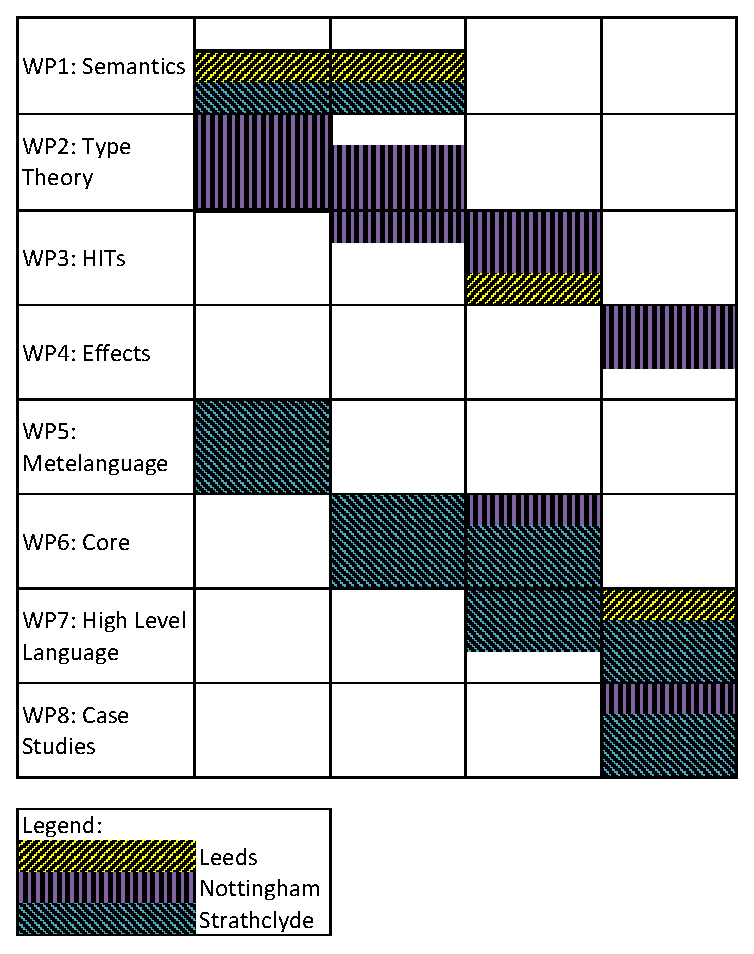
\includegraphics{Gantt.eps}
%\caption{Gantt chart depicting the order and division of work on workpackages}
%\end{figure}
%\newpage

\begin{footnotesize}
\begin{multicols}{2}
\bibliographystyle{plain}
%\bibliographystyle{abbrv}
%\bibliographystyle{plainnat}
\bibliography{proposal,alti,nicola}
\end{multicols}
\end{footnotesize}

% \begin{multicols}{2}
% \bibliographystyle{plain}
% \bibliography{proposal,alti}
% \end{multicols}{2}

\end{document}
